% !TEX encoding = UTF-8 Unicode
\level{2}{Fase DI: Documentation Improvement}
\textbf{Periodo}: dal \insdate{16}{02}{2015} al \insdate{05}{03}{2015} \\
Questa fase comincia al termine della \insphase{Fase DB}. È caratterizzata da una nuova analisi di tutti i documenti redatti nella fase precedente e dalla correzione di questi in base alle richieste e segnalazioni del committente. Gli analisti provvedono, inoltre, all'individuazione di nuovi requisiti e alla correzione di quelli segnalati. Pertanto, i documenti vengono ampliati ed aggiornati alla versione 2.00.
\level{3}{Diagramma di Gantt delle attività}
\begin{center}
	\begin{figure}[H]\centering
		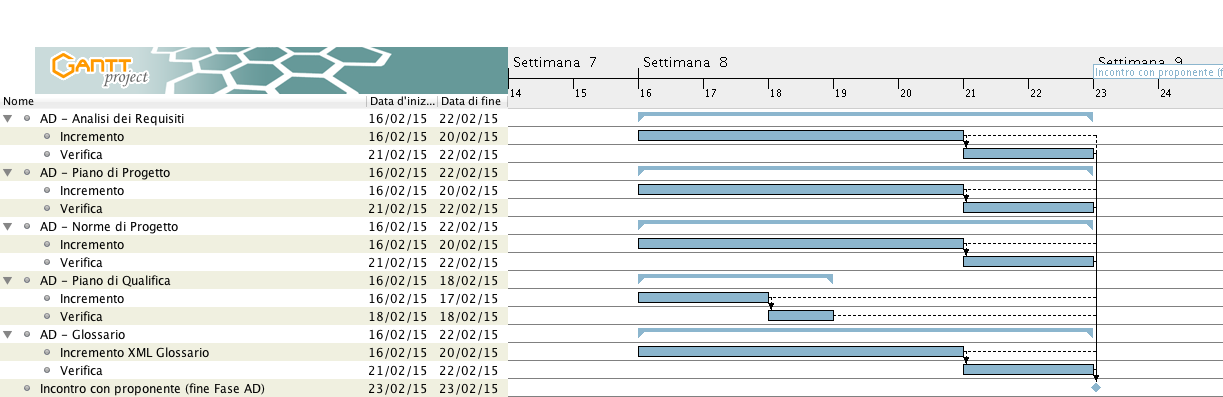
\includegraphics[width=\textwidth]{PianoDiProgetto/Pics/FaseDI.png}
		\caption{Gantt Fase DI}
	\end{figure}
\end{center}
